% Options for packages loaded elsewhere
\PassOptionsToPackage{unicode}{hyperref}
\PassOptionsToPackage{hyphens}{url}
%
\documentclass[
]{article}
\usepackage{amsmath,amssymb}
\usepackage{lmodern}
\usepackage{iftex}
\ifPDFTeX
  \usepackage[T1]{fontenc}
  \usepackage[utf8]{inputenc}
  \usepackage{textcomp} % provide euro and other symbols
\else % if luatex or xetex
  \usepackage{unicode-math}
  \defaultfontfeatures{Scale=MatchLowercase}
  \defaultfontfeatures[\rmfamily]{Ligatures=TeX,Scale=1}
\fi
% Use upquote if available, for straight quotes in verbatim environments
\IfFileExists{upquote.sty}{\usepackage{upquote}}{}
\IfFileExists{microtype.sty}{% use microtype if available
  \usepackage[]{microtype}
  \UseMicrotypeSet[protrusion]{basicmath} % disable protrusion for tt fonts
}{}
\makeatletter
\@ifundefined{KOMAClassName}{% if non-KOMA class
  \IfFileExists{parskip.sty}{%
    \usepackage{parskip}
  }{% else
    \setlength{\parindent}{0pt}
    \setlength{\parskip}{6pt plus 2pt minus 1pt}}
}{% if KOMA class
  \KOMAoptions{parskip=half}}
\makeatother
\usepackage{xcolor}
\IfFileExists{xurl.sty}{\usepackage{xurl}}{} % add URL line breaks if available
\IfFileExists{bookmark.sty}{\usepackage{bookmark}}{\usepackage{hyperref}}
\hypersetup{
  pdftitle={R Notebook},
  hidelinks,
  pdfcreator={LaTeX via pandoc}}
\urlstyle{same} % disable monospaced font for URLs
\usepackage[margin=1in]{geometry}
\usepackage{color}
\usepackage{fancyvrb}
\newcommand{\VerbBar}{|}
\newcommand{\VERB}{\Verb[commandchars=\\\{\}]}
\DefineVerbatimEnvironment{Highlighting}{Verbatim}{commandchars=\\\{\}}
% Add ',fontsize=\small' for more characters per line
\usepackage{framed}
\definecolor{shadecolor}{RGB}{248,248,248}
\newenvironment{Shaded}{\begin{snugshade}}{\end{snugshade}}
\newcommand{\AlertTok}[1]{\textcolor[rgb]{0.94,0.16,0.16}{#1}}
\newcommand{\AnnotationTok}[1]{\textcolor[rgb]{0.56,0.35,0.01}{\textbf{\textit{#1}}}}
\newcommand{\AttributeTok}[1]{\textcolor[rgb]{0.77,0.63,0.00}{#1}}
\newcommand{\BaseNTok}[1]{\textcolor[rgb]{0.00,0.00,0.81}{#1}}
\newcommand{\BuiltInTok}[1]{#1}
\newcommand{\CharTok}[1]{\textcolor[rgb]{0.31,0.60,0.02}{#1}}
\newcommand{\CommentTok}[1]{\textcolor[rgb]{0.56,0.35,0.01}{\textit{#1}}}
\newcommand{\CommentVarTok}[1]{\textcolor[rgb]{0.56,0.35,0.01}{\textbf{\textit{#1}}}}
\newcommand{\ConstantTok}[1]{\textcolor[rgb]{0.00,0.00,0.00}{#1}}
\newcommand{\ControlFlowTok}[1]{\textcolor[rgb]{0.13,0.29,0.53}{\textbf{#1}}}
\newcommand{\DataTypeTok}[1]{\textcolor[rgb]{0.13,0.29,0.53}{#1}}
\newcommand{\DecValTok}[1]{\textcolor[rgb]{0.00,0.00,0.81}{#1}}
\newcommand{\DocumentationTok}[1]{\textcolor[rgb]{0.56,0.35,0.01}{\textbf{\textit{#1}}}}
\newcommand{\ErrorTok}[1]{\textcolor[rgb]{0.64,0.00,0.00}{\textbf{#1}}}
\newcommand{\ExtensionTok}[1]{#1}
\newcommand{\FloatTok}[1]{\textcolor[rgb]{0.00,0.00,0.81}{#1}}
\newcommand{\FunctionTok}[1]{\textcolor[rgb]{0.00,0.00,0.00}{#1}}
\newcommand{\ImportTok}[1]{#1}
\newcommand{\InformationTok}[1]{\textcolor[rgb]{0.56,0.35,0.01}{\textbf{\textit{#1}}}}
\newcommand{\KeywordTok}[1]{\textcolor[rgb]{0.13,0.29,0.53}{\textbf{#1}}}
\newcommand{\NormalTok}[1]{#1}
\newcommand{\OperatorTok}[1]{\textcolor[rgb]{0.81,0.36,0.00}{\textbf{#1}}}
\newcommand{\OtherTok}[1]{\textcolor[rgb]{0.56,0.35,0.01}{#1}}
\newcommand{\PreprocessorTok}[1]{\textcolor[rgb]{0.56,0.35,0.01}{\textit{#1}}}
\newcommand{\RegionMarkerTok}[1]{#1}
\newcommand{\SpecialCharTok}[1]{\textcolor[rgb]{0.00,0.00,0.00}{#1}}
\newcommand{\SpecialStringTok}[1]{\textcolor[rgb]{0.31,0.60,0.02}{#1}}
\newcommand{\StringTok}[1]{\textcolor[rgb]{0.31,0.60,0.02}{#1}}
\newcommand{\VariableTok}[1]{\textcolor[rgb]{0.00,0.00,0.00}{#1}}
\newcommand{\VerbatimStringTok}[1]{\textcolor[rgb]{0.31,0.60,0.02}{#1}}
\newcommand{\WarningTok}[1]{\textcolor[rgb]{0.56,0.35,0.01}{\textbf{\textit{#1}}}}
\usepackage{graphicx}
\makeatletter
\def\maxwidth{\ifdim\Gin@nat@width>\linewidth\linewidth\else\Gin@nat@width\fi}
\def\maxheight{\ifdim\Gin@nat@height>\textheight\textheight\else\Gin@nat@height\fi}
\makeatother
% Scale images if necessary, so that they will not overflow the page
% margins by default, and it is still possible to overwrite the defaults
% using explicit options in \includegraphics[width, height, ...]{}
\setkeys{Gin}{width=\maxwidth,height=\maxheight,keepaspectratio}
% Set default figure placement to htbp
\makeatletter
\def\fps@figure{htbp}
\makeatother
\setlength{\emergencystretch}{3em} % prevent overfull lines
\providecommand{\tightlist}{%
  \setlength{\itemsep}{0pt}\setlength{\parskip}{0pt}}
\setcounter{secnumdepth}{-\maxdimen} % remove section numbering
\ifLuaTeX
  \usepackage{selnolig}  % disable illegal ligatures
\fi

\title{R Notebook}
\author{}
\date{\vspace{-2.5em}}

\begin{document}
\maketitle

\begin{description}
\tightlist
\item[Let us have a look at an example where using a nonlinear
regression function is better suited for estimating the population
relationship between the regressor, \(X\), and the regressand, \(Y\)]
the relationship between the income of schooling districts and their
test scores.
\end{description}

\begin{Shaded}
\begin{Highlighting}[]
\CommentTok{\# prepare the data}
\FunctionTok{library}\NormalTok{(AER)                                                     }
\FunctionTok{data}\NormalTok{(CASchools)}
\NormalTok{CASchools}\SpecialCharTok{$}\NormalTok{size }\OtherTok{\textless{}{-}}\NormalTok{ CASchools}\SpecialCharTok{$}\NormalTok{students}\SpecialCharTok{/}\NormalTok{CASchools}\SpecialCharTok{$}\NormalTok{teachers}
\NormalTok{CASchools}\SpecialCharTok{$}\NormalTok{score }\OtherTok{\textless{}{-}}\NormalTok{ (CASchools}\SpecialCharTok{$}\NormalTok{read }\SpecialCharTok{+}\NormalTok{ CASchools}\SpecialCharTok{$}\NormalTok{math) }\SpecialCharTok{/} \DecValTok{2}
\end{Highlighting}
\end{Shaded}

We start our analysis by computing the correlation between both
variables.

\begin{Shaded}
\begin{Highlighting}[]
\FunctionTok{cor}\NormalTok{(CASchools}\SpecialCharTok{$}\NormalTok{income, CASchools}\SpecialCharTok{$}\NormalTok{score)}
\end{Highlighting}
\end{Shaded}

\begin{verbatim}
## [1] 0.7124308
\end{verbatim}

\begin{Shaded}
\begin{Highlighting}[]
\CommentTok{\# fit a simple linear model}
\NormalTok{linear\_model}\OtherTok{\textless{}{-}} \FunctionTok{lm}\NormalTok{(score }\SpecialCharTok{\textasciitilde{}}\NormalTok{ income, }\AttributeTok{data =}\NormalTok{ CASchools)}

\CommentTok{\# plot the observations}
\FunctionTok{plot}\NormalTok{(CASchools}\SpecialCharTok{$}\NormalTok{income, CASchools}\SpecialCharTok{$}\NormalTok{score,}
     \AttributeTok{col =} \StringTok{"steelblue"}\NormalTok{,}
     \AttributeTok{pch =} \DecValTok{20}\NormalTok{,}
     \AttributeTok{xlab =} \StringTok{"District Income (thousands of dollars)"}\NormalTok{, }
     \AttributeTok{ylab =} \StringTok{"Test Score"}\NormalTok{,}
     \AttributeTok{cex.main =} \FloatTok{0.9}\NormalTok{,}
     \AttributeTok{main =} \StringTok{"Test Score vs. District Income and a Linear OLS Regression Function"}\NormalTok{)}

\CommentTok{\# add the regression line to the plot}
\FunctionTok{abline}\NormalTok{(linear\_model, }
       \AttributeTok{col =} \StringTok{"red"}\NormalTok{, }
       \AttributeTok{lwd =} \DecValTok{2}\NormalTok{)}
\end{Highlighting}
\end{Shaded}

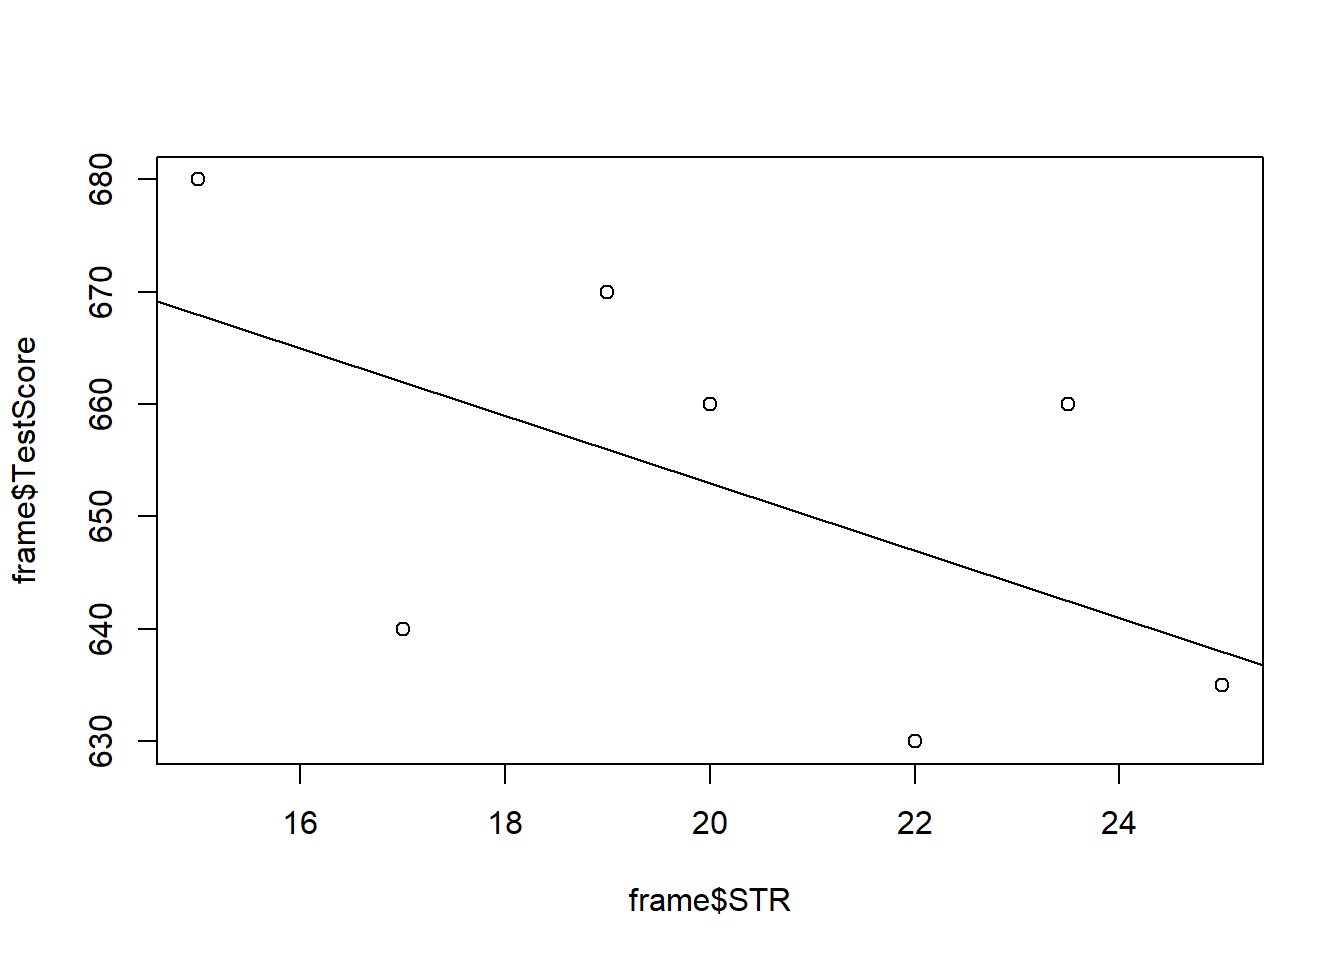
\includegraphics{5_nonlinear_regression_files/figure-latex/unnamed-chunk-3-1.pdf}

Fortunately, OLS does not only handle linear functions of the
regressors. We can for example model test scores as a function of income
and the square of income. The corresponding regression model is

\[TestScore_i = \beta_0 + \beta_1 \times income_i + \beta_2 \times income_i^2 + u_i,\]
called a \emph{quadratic regression model}. That is, \(income^2\) is
treated as an additional explanatory variable. Hence, the quadratic
model is a special case of a multivariate regression model.

\begin{Shaded}
\begin{Highlighting}[]
\CommentTok{\# fit the quadratic Model}
\NormalTok{quadratic\_model }\OtherTok{\textless{}{-}} \FunctionTok{lm}\NormalTok{(score }\SpecialCharTok{\textasciitilde{}}\NormalTok{ income }\SpecialCharTok{+} \FunctionTok{I}\NormalTok{(income}\SpecialCharTok{\^{}}\DecValTok{2}\NormalTok{), }\AttributeTok{data =}\NormalTok{ CASchools)}

\CommentTok{\# obtain the model summary}
\FunctionTok{coeftest}\NormalTok{(quadratic\_model, }\AttributeTok{vcov. =}\NormalTok{ vcovHC, }\AttributeTok{type =} \StringTok{"HC1"}\NormalTok{)}
\end{Highlighting}
\end{Shaded}

\begin{verbatim}
## 
## t test of coefficients:
## 
##                Estimate  Std. Error  t value  Pr(>|t|)    
## (Intercept) 607.3017435   2.9017544 209.2878 < 2.2e-16 ***
## income        3.8509939   0.2680942  14.3643 < 2.2e-16 ***
## I(income^2)  -0.0423084   0.0047803  -8.8505 < 2.2e-16 ***
## ---
## Signif. codes:  0 '***' 0.001 '**' 0.01 '*' 0.05 '.' 0.1 ' ' 1
\end{verbatim}

The output tells us that the estimated regression function is

\[\widehat{TestScore}_i = \underset{(2.90)}{607.3} + \underset{(0.27)}{3.85} \times income_i - \underset{(0.0048)}{0.0423} \times income_i^2.\]

This model allows us to test the hypothesis that the relationship
between test scores and district income is linear against the
alternative that it is quadratic. This corresponds to testing

\[H_0: \beta_2 = 0 \ \ \text{vs.} \ \  H_1: \beta_2\neq0,\]

since \(\beta_2=0\) corresponds to a simple linear equation and
\(\beta_2\neq0\) implies a quadratic relationship. We find that
\(t=(\hat\beta_2 - 0)/SE(\hat\beta_2) = -0.0423/0.0048 = -8.81\) so the
null is rejected at any common level of significance and we conclude
that the relationship is nonlinear. This is consistent with the
impression gained from the plot.

\begin{Shaded}
\begin{Highlighting}[]
\CommentTok{\# draw a scatterplot of the observations for income and test score}
\FunctionTok{plot}\NormalTok{(CASchools}\SpecialCharTok{$}\NormalTok{income, CASchools}\SpecialCharTok{$}\NormalTok{score,}
     \AttributeTok{col  =} \StringTok{"steelblue"}\NormalTok{,}
     \AttributeTok{pch =} \DecValTok{20}\NormalTok{,}
     \AttributeTok{xlab =} \StringTok{"District Income (thousands of dollars)"}\NormalTok{,}
     \AttributeTok{ylab =} \StringTok{"Test Score"}\NormalTok{,}
     \AttributeTok{main =} \StringTok{"Estimated Linear and Quadratic Regression Functions"}\NormalTok{)}

\CommentTok{\# add a linear function to the plot}
\FunctionTok{abline}\NormalTok{(linear\_model, }\AttributeTok{col =} \StringTok{"black"}\NormalTok{, }\AttributeTok{lwd =} \DecValTok{2}\NormalTok{)}

\CommentTok{\# add quatratic function to the plot}
\NormalTok{order\_id }\OtherTok{\textless{}{-}} \FunctionTok{order}\NormalTok{(CASchools}\SpecialCharTok{$}\NormalTok{income)}

\FunctionTok{lines}\NormalTok{(}\AttributeTok{x =}\NormalTok{ CASchools}\SpecialCharTok{$}\NormalTok{income[order\_id], }
      \AttributeTok{y =} \FunctionTok{fitted}\NormalTok{(quadratic\_model)[order\_id],}
      \AttributeTok{col =} \StringTok{"red"}\NormalTok{, }
      \AttributeTok{lwd =} \DecValTok{2}\NormalTok{) }
\end{Highlighting}
\end{Shaded}

\begin{center}\includegraphics{5_nonlinear_regression_files/figure-latex/unnamed-chunk-5-1} \end{center}

We see that the quadratic function does fit the data much better than
the linear function.

\hypertarget{nfoasiv}{%
\subsection{Nonlinear Functions of a Single Independent
Variable}\label{nfoasiv}}

\hypertarget{polynomials}{%
\subsubsection*{Polynomials}\label{polynomials}}
\addcontentsline{toc}{subsubsection}{Polynomials}

The approach used to obtain a quadratic model can be generalized to
polynomial models of arbitrary degree \(r\),
\[Y_i = \beta_0 + \beta_1 X_i + \beta_2 X_i^2 + \cdots + \beta_r X_i^r + u_i.\]

A cubic model for instance can be estimated in the same way as the
quadratic model; we just have to use a polynomial of degree \(r=3\) in
\texttt{income}. This is conveniently done using the function
\texttt{poly()}.

\begin{Shaded}
\begin{Highlighting}[]
\CommentTok{\# estimate a cubic model}
\NormalTok{cubic\_model }\OtherTok{\textless{}{-}} \FunctionTok{lm}\NormalTok{(score }\SpecialCharTok{\textasciitilde{}} \FunctionTok{poly}\NormalTok{(income, }\AttributeTok{degree =} \DecValTok{3}\NormalTok{, }\AttributeTok{raw =} \ConstantTok{TRUE}\NormalTok{), }\AttributeTok{data =}\NormalTok{ CASchools)}
\end{Highlighting}
\end{Shaded}

\texttt{poly()} generates orthogonal polynomials which are orthogonal to
the constant by default. Here, we set \texttt{"raw\ =\ TRUE} such that
raw polynomials are evaluated, see \texttt{?poly}.

In practice the question will arise which polynomial order should be
chosen. First, similarly as for \(r=2\), we can test the null hypothesis
that the true relation is linear against the alternative hypothesis that
the relationship is a polynomial of degree \(r\):

\[ H_0: \beta_2=0, \ \beta_3=0,\dots,\beta_r=0 \ \ \ \text{vs.} \ \ \ H_1: \text{at least one} \ \beta_j\neq0, \ j=2,\dots,r \]

This is a joint null hypothesis with \(r-1\) restrictions so it can be
tested using the \(F\)-test presented in Chapter @ref(htaciimr).
\texttt{linearHypothesis()} can be used to conduct such tests. For
example, we may test the null of a linear model against the alternative
of a polynomial of a maximal degree \(r=3\) as follows.

\begin{Shaded}
\begin{Highlighting}[]
\CommentTok{\# test the hypothesis of a linear model against quadratic or polynomial}
\CommentTok{\# alternatives}

\CommentTok{\# set up hypothesis matrix}
\NormalTok{R }\OtherTok{\textless{}{-}} \FunctionTok{rbind}\NormalTok{(}\FunctionTok{c}\NormalTok{(}\DecValTok{0}\NormalTok{, }\DecValTok{0}\NormalTok{, }\DecValTok{1}\NormalTok{, }\DecValTok{0}\NormalTok{),}
            \FunctionTok{c}\NormalTok{(}\DecValTok{0}\NormalTok{, }\DecValTok{0}\NormalTok{, }\DecValTok{0}\NormalTok{, }\DecValTok{1}\NormalTok{))}

\CommentTok{\# do the test}
\FunctionTok{linearHypothesis}\NormalTok{(cubic\_model,}
                 \AttributeTok{hypothesis.matrix =}\NormalTok{ R,}
                 \AttributeTok{white.adj =} \StringTok{"hc1"}\NormalTok{)}
\end{Highlighting}
\end{Shaded}

\begin{verbatim}
## Linear hypothesis test
## 
## Hypothesis:
## poly(income, degree = 3, raw = TRUE)2 = 0
## poly(income, degree = 3, raw = TRUE)3 = 0
## 
## Model 1: restricted model
## Model 2: score ~ poly(income, degree = 3, raw = TRUE)
## 
## Note: Coefficient covariance matrix supplied.
## 
##   Res.Df Df      F    Pr(>F)    
## 1    418                        
## 2    416  2 37.691 9.043e-16 ***
## ---
## Signif. codes:  0 '***' 0.001 '**' 0.01 '*' 0.05 '.' 0.1 ' ' 1
\end{verbatim}

For the two linear constrains above, we have \begin{align*}
  \mathbf{R}\boldsymbol{\beta} =& \mathbf{s} \\
  \begin{pmatrix}
    0 & 0 & 1 & 0 \\
    0 & 0 & 0 & 1
  \end{pmatrix}
  \begin{pmatrix}
    \beta_0 \\
    \beta_1 \\
    \beta_2 \\
    \beta_3 \\
  \end{pmatrix} =&
  \begin{pmatrix}
   0 \\
   0
  \end{pmatrix} \\
  \begin{pmatrix}
    \beta_2 \\
    \beta_3
  \end{pmatrix}= &
  \begin{pmatrix}
    0 \\
    0
  \end{pmatrix}.
\end{align*} \texttt{linearHypothesis()} uses the zero vector for
\(\mathbf{s}\) by default, see \texttt{?linearHypothesis}.

The \(p\)-value for is very small so that we reject the null hypothesis.
However, this does not tell us \emph{which} \(r\) to choose. In
practice, one approach to determine the degree of the polynomial is to
use \emph{sequential testing}:

\begin{enumerate}
\def\labelenumi{\arabic{enumi}.}
\tightlist
\item
  Estimate a polynomial model for some maximum value \(r\).
\item
  Use a \(t\)-test to test \(\beta_r = 0\). \emph{Rejection} of the null
  means that \(X^r\) belongs in the regression equation.
\item
  \emph{Acceptance} of the null in step 2 means that \(X^r\) can be
  eliminated from the model. Continue by repeating step 1 with order
  \(r-1\) and test whether \(\beta_{r-1}=0\). If the test rejects, use a
  polynomial model of order \(r-1\).
\item
  If the tests from step 3 rejects, continue with the procedure until
  the coefficient on the highest power is statistically significant.
\end{enumerate}

There is no unambiguous guideline how to choose \(r\) in step one.
However, as pointed out in @stock2015, economic data is often smooth
such that it is appropriate to choose small orders like \(2\), \(3\), or
\(4\).

We will demonstrate how to apply sequential testing by the example of
the cubic model.

\begin{Shaded}
\begin{Highlighting}[]
\FunctionTok{summary}\NormalTok{(cubic\_model)}
\end{Highlighting}
\end{Shaded}

\begin{verbatim}
## 
## Call:
## lm(formula = score ~ poly(income, degree = 3, raw = TRUE), data = CASchools)
## 
## Residuals:
##    Min     1Q Median     3Q    Max 
## -44.28  -9.21   0.20   8.32  31.16 
## 
## Coefficients:
##                                         Estimate Std. Error t value Pr(>|t|)
## (Intercept)                            6.001e+02  5.830e+00 102.937  < 2e-16
## poly(income, degree = 3, raw = TRUE)1  5.019e+00  8.595e-01   5.839 1.06e-08
## poly(income, degree = 3, raw = TRUE)2 -9.581e-02  3.736e-02  -2.564   0.0107
## poly(income, degree = 3, raw = TRUE)3  6.855e-04  4.720e-04   1.452   0.1471
##                                          
## (Intercept)                           ***
## poly(income, degree = 3, raw = TRUE)1 ***
## poly(income, degree = 3, raw = TRUE)2 *  
## poly(income, degree = 3, raw = TRUE)3    
## ---
## Signif. codes:  0 '***' 0.001 '**' 0.01 '*' 0.05 '.' 0.1 ' ' 1
## 
## Residual standard error: 12.71 on 416 degrees of freedom
## Multiple R-squared:  0.5584, Adjusted R-squared:  0.5552 
## F-statistic: 175.4 on 3 and 416 DF,  p-value: < 2.2e-16
\end{verbatim}

The \(t\)-statistic on \(income^3\) is \(1.42\) so the null that the
relationship is quadratic cannot be rejected, even at the \(10\%\)
level. This is contrary to the result presented book which reports
robust standard errors throughout so we will also use robust
variance-covariance estimation to reproduce these results.

\begin{Shaded}
\begin{Highlighting}[]
\CommentTok{\# test the hypothesis using robust standard errors}
\FunctionTok{coeftest}\NormalTok{(cubic\_model, }\AttributeTok{vcov. =}\NormalTok{ vcovHC, }\AttributeTok{type =} \StringTok{"HC1"}\NormalTok{)}
\end{Highlighting}
\end{Shaded}

\begin{verbatim}
## 
## t test of coefficients:
## 
##                                          Estimate  Std. Error  t value
## (Intercept)                            6.0008e+02  5.1021e+00 117.6150
## poly(income, degree = 3, raw = TRUE)1  5.0187e+00  7.0735e-01   7.0950
## poly(income, degree = 3, raw = TRUE)2 -9.5805e-02  2.8954e-02  -3.3089
## poly(income, degree = 3, raw = TRUE)3  6.8549e-04  3.4706e-04   1.9751
##                                        Pr(>|t|)    
## (Intercept)                           < 2.2e-16 ***
## poly(income, degree = 3, raw = TRUE)1 5.606e-12 ***
## poly(income, degree = 3, raw = TRUE)2  0.001018 ** 
## poly(income, degree = 3, raw = TRUE)3  0.048918 *  
## ---
## Signif. codes:  0 '***' 0.001 '**' 0.01 '*' 0.05 '.' 0.1 ' ' 1
\end{verbatim}

\begin{Shaded}
\begin{Highlighting}[]
\CommentTok{\# perform robust F{-}test }
\FunctionTok{linearHypothesis}\NormalTok{(cubic\_model, }
                 \AttributeTok{hypothesis.matrix =}\NormalTok{ R,}
                 \AttributeTok{vcov. =}\NormalTok{ vcovHC, }\AttributeTok{type =} \StringTok{"HC1"}\NormalTok{)}
\end{Highlighting}
\end{Shaded}

\begin{verbatim}
## Linear hypothesis test
## 
## Hypothesis:
## poly(income, degree = 3, raw = TRUE)2 = 0
## poly(income, degree = 3, raw = TRUE)3 = 0
## 
## Model 1: restricted model
## Model 2: score ~ poly(income, degree = 3, raw = TRUE)
## 
## Note: Coefficient covariance matrix supplied.
## 
##   Res.Df Df      F    Pr(>F)    
## 1    418                        
## 2    416  2 29.678 8.945e-13 ***
## ---
## Signif. codes:  0 '***' 0.001 '**' 0.01 '*' 0.05 '.' 0.1 ' ' 1
\end{verbatim}

With a \(p\)-value of \(9.043e^{-16}\), i.e., much less than \(0.05\),
the null hypothesis of linearity is rejected in favor of the alternative
that the relationship is quadratic \emph{or} cubic.

\hypertarget{prediction-of-marginal-effect-of-income}{%
\subsubsection{Prediction of Marginal Effect of
Income}\label{prediction-of-marginal-effect-of-income}}

Because the regression function is quadratic, this effect depends on the
\emph{initial} district income. We therefore consider two cases:

\begin{enumerate}
\def\labelenumi{\arabic{enumi}.}
\item
  An increase in district income form \(10\) to \(11\) (from \(\$10000\)
  per capita to \(\$11000\)).
\item
  An increase in district income from \(40\) to \(41\) (that is from
  \(\$40000\) to \(\$41000\)).
\end{enumerate}

In order to obtain the \(\Delta \widehat{Y}\) associated with a change
in income form \(10\) to \(11\), we use the following formula:

\[\Delta \widehat{Y} = \left(\hat{\beta}_0 + \hat{\beta}_1 \times 11 + \hat{\beta}_2 \times 11^2\right) - \left(\hat{\beta}_0 + \hat{\beta}_1 \times 10 + \hat{\beta}_2 \times 10^2\right) \]

\begin{Shaded}
\begin{Highlighting}[]
\CommentTok{\# compute and assign the quadratic model}
\NormalTok{quadriatic\_model }\OtherTok{\textless{}{-}} \FunctionTok{lm}\NormalTok{(score }\SpecialCharTok{\textasciitilde{}}\NormalTok{ income }\SpecialCharTok{+} \FunctionTok{I}\NormalTok{(income}\SpecialCharTok{\^{}}\DecValTok{2}\NormalTok{), }\AttributeTok{data =}\NormalTok{ CASchools)}

\CommentTok{\# set up data for prediction}
\NormalTok{new\_data }\OtherTok{\textless{}{-}} \FunctionTok{data.frame}\NormalTok{(}\AttributeTok{income =} \FunctionTok{c}\NormalTok{(}\DecValTok{10}\NormalTok{, }\DecValTok{11}\NormalTok{))}

\CommentTok{\# do the prediction}
\NormalTok{Y\_hat }\OtherTok{\textless{}{-}} \FunctionTok{predict}\NormalTok{(quadriatic\_model, }\AttributeTok{newdata =}\NormalTok{ new\_data)}

\CommentTok{\# compute the difference}
\FunctionTok{diff}\NormalTok{(Y\_hat)}
\end{Highlighting}
\end{Shaded}

\begin{verbatim}
##        2 
## 2.962517
\end{verbatim}

Analogously we can compute the effect of a change in district income
from \(40\) to \(41\):

\begin{Shaded}
\begin{Highlighting}[]
\CommentTok{\# set up data for prediction}
\NormalTok{new\_data }\OtherTok{\textless{}{-}} \FunctionTok{data.frame}\NormalTok{(}\AttributeTok{income =} \FunctionTok{c}\NormalTok{(}\DecValTok{40}\NormalTok{, }\DecValTok{41}\NormalTok{))}

\CommentTok{\# do the prediction}
\NormalTok{Y\_hat }\OtherTok{\textless{}{-}} \FunctionTok{predict}\NormalTok{(quadriatic\_model, }\AttributeTok{newdata =}\NormalTok{ new\_data)}

\CommentTok{\# compute the difference}
\FunctionTok{diff}\NormalTok{(Y\_hat)}
\end{Highlighting}
\end{Shaded}

\begin{verbatim}
##         2 
## 0.4240097
\end{verbatim}

\hypertarget{logarithms}{%
\subsubsection*{Logarithms}\label{logarithms}}
\addcontentsline{toc}{subsubsection}{Logarithms}

Another way to specify a nonlinear regression function is to use the
natural logarithm of \(Y\) and/or \(X\). Logarithms convert changes in
variables into percentage changes. This is convenient as many
relationships are naturally expressed in terms of percentages.

\hypertarget{case-i-x-is-in-logarithm-y-is-not.}{%
\paragraph*{\texorpdfstring{Case I: \(X\) is in Logarithm, \(Y\) is
not.}{Case I: X is in Logarithm, Y is not.}}\label{case-i-x-is-in-logarithm-y-is-not.}}
\addcontentsline{toc}{paragraph}{Case I: \(X\) is in Logarithm, \(Y\) is
not.}

The regression model then is
\[Y_i = \beta_0 + \beta_1 \times \ln(X_i) + u_i \text{, } i=1,...,n. \]
Similar as for polynomial regression we do not have to create a new
variable before using \texttt{lm()}.

\begin{Shaded}
\begin{Highlighting}[]
\CommentTok{\# estimate a level{-}log model}
\NormalTok{LinearLog\_model }\OtherTok{\textless{}{-}} \FunctionTok{lm}\NormalTok{(score }\SpecialCharTok{\textasciitilde{}} \FunctionTok{log}\NormalTok{(income), }\AttributeTok{data =}\NormalTok{ CASchools)}

\CommentTok{\# compute robust summary}
\FunctionTok{coeftest}\NormalTok{(LinearLog\_model, }
         \AttributeTok{vcov =}\NormalTok{ vcovHC, }\AttributeTok{type =} \StringTok{"HC1"}\NormalTok{)}
\end{Highlighting}
\end{Shaded}

\begin{verbatim}
## 
## t test of coefficients:
## 
##             Estimate Std. Error t value  Pr(>|t|)    
## (Intercept) 557.8323     3.8399 145.271 < 2.2e-16 ***
## log(income)  36.4197     1.3969  26.071 < 2.2e-16 ***
## ---
## Signif. codes:  0 '***' 0.001 '**' 0.01 '*' 0.05 '.' 0.1 ' ' 1
\end{verbatim}

Hence, the estimated regression function is

\[\widehat{TestScore} = 557.8 + 36.42 \times \ln(income).\]

Let us draw a plot of this function.

\begin{Shaded}
\begin{Highlighting}[]
\CommentTok{\# draw a scatterplot}
\FunctionTok{plot}\NormalTok{(score }\SpecialCharTok{\textasciitilde{}}\NormalTok{ income, }
     \AttributeTok{col =} \StringTok{"steelblue"}\NormalTok{,}
     \AttributeTok{pch =} \DecValTok{20}\NormalTok{,}
     \AttributeTok{data =}\NormalTok{ CASchools,}
     \AttributeTok{main =} \StringTok{"Linear{-}Log Regression Line"}\NormalTok{)}

\CommentTok{\# add the linear{-}log regression line}
\NormalTok{order\_id  }\OtherTok{\textless{}{-}} \FunctionTok{order}\NormalTok{(CASchools}\SpecialCharTok{$}\NormalTok{income)}

\FunctionTok{lines}\NormalTok{(CASchools}\SpecialCharTok{$}\NormalTok{income[order\_id],}
      \FunctionTok{fitted}\NormalTok{(LinearLog\_model)[order\_id], }
      \AttributeTok{col =} \StringTok{"red"}\NormalTok{, }
      \AttributeTok{lwd =} \DecValTok{2}\NormalTok{)}
\end{Highlighting}
\end{Shaded}

\begin{center}\includegraphics{5_nonlinear_regression_files/figure-latex/unnamed-chunk-11-1} \end{center}

We can interpret \(\hat{\beta}_1\) as follows: a \(1\%\) increase in
income is associated with an increase in test scores of
\(0.01 \times 36.42 = 0.36\) points. In order to get the estimated
effect of a one unit change in income (that is, a change in the original
units, thousands of dollars) on test scores, the method presented in Key
Concept 8.1 can be used.

\begin{Shaded}
\begin{Highlighting}[]
\CommentTok{\# set up new data}
\NormalTok{new\_data }\OtherTok{\textless{}{-}} \FunctionTok{data.frame}\NormalTok{(}\AttributeTok{income =} \FunctionTok{c}\NormalTok{(}\DecValTok{10}\NormalTok{, }\DecValTok{11}\NormalTok{, }\DecValTok{40}\NormalTok{, }\DecValTok{41}\NormalTok{))}

\CommentTok{\# predict the outcomes }
\NormalTok{Y\_hat }\OtherTok{\textless{}{-}} \FunctionTok{predict}\NormalTok{(LinearLog\_model, }\AttributeTok{newdata =}\NormalTok{ new\_data)}

\CommentTok{\# compute the expected difference}
\NormalTok{Y\_hat\_matrix }\OtherTok{\textless{}{-}} \FunctionTok{matrix}\NormalTok{(Y\_hat, }\AttributeTok{nrow =} \DecValTok{2}\NormalTok{, }\AttributeTok{byrow =} \ConstantTok{TRUE}\NormalTok{)}
\NormalTok{Y\_hat\_matrix[, }\DecValTok{2}\NormalTok{] }\SpecialCharTok{{-}}\NormalTok{ Y\_hat\_matrix[, }\DecValTok{1}\NormalTok{]}
\end{Highlighting}
\end{Shaded}

\begin{verbatim}
## [1] 3.471166 0.899297
\end{verbatim}

\hypertarget{case-ii-y-is-in-logarithm-x-is-not}{%
\paragraph*{\texorpdfstring{Case II: \(Y\) is in Logarithm, \(X\) is
not}{Case II: Y is in Logarithm, X is not}}\label{case-ii-y-is-in-logarithm-x-is-not}}
\addcontentsline{toc}{paragraph}{Case II: \(Y\) is in Logarithm, \(X\)
is not}

There are cases where it is useful to regress \(\ln(Y)\).

The corresponding regression model then is

\[ \ln(Y_i) = \beta_0 + \beta_1 \times X_i + u_i , \ \ i=1,...,n. \]

\begin{Shaded}
\begin{Highlighting}[]
\CommentTok{\# estimate a log{-}linear model }
\NormalTok{LogLinear\_model }\OtherTok{\textless{}{-}} \FunctionTok{lm}\NormalTok{(}\FunctionTok{log}\NormalTok{(score) }\SpecialCharTok{\textasciitilde{}}\NormalTok{ income, }\AttributeTok{data =}\NormalTok{ CASchools)}

\CommentTok{\# obtain a robust coefficient summary}
\FunctionTok{coeftest}\NormalTok{(LogLinear\_model, }
         \AttributeTok{vcov =}\NormalTok{ vcovHC, }\AttributeTok{type =} \StringTok{"HC1"}\NormalTok{)}
\end{Highlighting}
\end{Shaded}

\begin{verbatim}
## 
## t test of coefficients:
## 
##               Estimate Std. Error  t value  Pr(>|t|)    
## (Intercept) 6.43936234 0.00289382 2225.210 < 2.2e-16 ***
## income      0.00284407 0.00017509   16.244 < 2.2e-16 ***
## ---
## Signif. codes:  0 '***' 0.001 '**' 0.01 '*' 0.05 '.' 0.1 ' ' 1
\end{verbatim}

The estimated regression function is
\[\widehat{\ln(TestScore)} = 6.439 + 0.00284 \times income.\] An
increase in district income by \(\$1000\) is expected to increase test
scores by \(100\times 0.00284 \% = 0.284\%\).

When the dependent variable in logarithm, one cannot simply use
\(e^{\log(\cdot)}\) to transform predictions back to the original scale,
see page of the book.

\hypertarget{case-iii-x-and-y-are-in-logarithms}{%
\paragraph*{\texorpdfstring{Case III: \(X\) and \(Y\) are in
Logarithms}{Case III: X and Y are in Logarithms}}\label{case-iii-x-and-y-are-in-logarithms}}
\addcontentsline{toc}{paragraph}{Case III: \(X\) and \(Y\) are in
Logarithms}

The log-log regression model is
\[\ln(Y_i) = \beta_0 + \beta_1 \times \ln(X_i) + u_i, \ \ i=1,...,n.\]

\begin{Shaded}
\begin{Highlighting}[]
\CommentTok{\# estimate the log{-}log model}
\NormalTok{LogLog\_model }\OtherTok{\textless{}{-}} \FunctionTok{lm}\NormalTok{(}\FunctionTok{log}\NormalTok{(score) }\SpecialCharTok{\textasciitilde{}} \FunctionTok{log}\NormalTok{(income), }\AttributeTok{data =}\NormalTok{ CASchools)}

\CommentTok{\# print robust coefficient summary to the console}
\FunctionTok{coeftest}\NormalTok{(LogLog\_model, }
         \AttributeTok{vcov =}\NormalTok{ vcovHC, }\AttributeTok{type =} \StringTok{"HC1"}\NormalTok{)}
\end{Highlighting}
\end{Shaded}

\begin{verbatim}
## 
## t test of coefficients:
## 
##              Estimate Std. Error  t value  Pr(>|t|)    
## (Intercept) 6.3363494  0.0059246 1069.501 < 2.2e-16 ***
## log(income) 0.0554190  0.0021446   25.841 < 2.2e-16 ***
## ---
## Signif. codes:  0 '***' 0.001 '**' 0.01 '*' 0.05 '.' 0.1 ' ' 1
\end{verbatim}

The estimated regression function hence is
\[\widehat{\ln(TestScore)} = 6.336 + 0.0554 \times \ln(income).\] In a
log-log model, a \(1\%\) change in \(X\) is associated with an estimated
\(\hat\beta_1 \%\) change in \(Y\).

We now reproduce Figure 8.5 of the book.

\begin{Shaded}
\begin{Highlighting}[]
\CommentTok{\# generate a scatterplot}
\FunctionTok{plot}\NormalTok{(}\FunctionTok{log}\NormalTok{(score) }\SpecialCharTok{\textasciitilde{}}\NormalTok{ income, }
     \AttributeTok{col =} \StringTok{"steelblue"}\NormalTok{, }
     \AttributeTok{pch =} \DecValTok{20}\NormalTok{, }
     \AttributeTok{data =}\NormalTok{ CASchools,}
     \AttributeTok{main =} \StringTok{"Log{-}Linear Regression Function"}\NormalTok{)}

\CommentTok{\# add the log{-}linear regression line}
\NormalTok{order\_id  }\OtherTok{\textless{}{-}} \FunctionTok{order}\NormalTok{(CASchools}\SpecialCharTok{$}\NormalTok{income)}

\FunctionTok{lines}\NormalTok{(CASchools}\SpecialCharTok{$}\NormalTok{income[order\_id], }
      \FunctionTok{fitted}\NormalTok{(LogLinear\_model)[order\_id], }
      \AttributeTok{col =} \StringTok{"red"}\NormalTok{, }
      \AttributeTok{lwd =} \DecValTok{2}\NormalTok{)}

\CommentTok{\# add the log{-}log regression line}
\FunctionTok{lines}\NormalTok{(}\FunctionTok{sort}\NormalTok{(CASchools}\SpecialCharTok{$}\NormalTok{income), }
      \FunctionTok{fitted}\NormalTok{(LogLog\_model)[}\FunctionTok{order}\NormalTok{(CASchools}\SpecialCharTok{$}\NormalTok{income)], }
      \AttributeTok{col =} \StringTok{"green"}\NormalTok{, }
      \AttributeTok{lwd =} \DecValTok{2}\NormalTok{)}

\CommentTok{\# add a legend}
\FunctionTok{legend}\NormalTok{(}\StringTok{"bottomright"}\NormalTok{,}
       \AttributeTok{legend =} \FunctionTok{c}\NormalTok{(}\StringTok{"log{-}linear model"}\NormalTok{, }\StringTok{"log{-}log model"}\NormalTok{),}
       \AttributeTok{lwd =} \DecValTok{2}\NormalTok{,}
       \AttributeTok{col =} \FunctionTok{c}\NormalTok{(}\StringTok{"red"}\NormalTok{, }\StringTok{"green"}\NormalTok{))}
\end{Highlighting}
\end{Shaded}

\begin{center}\includegraphics{5_nonlinear_regression_files/figure-latex/unnamed-chunk-14-1} \end{center}

Of course we can also estimate a \emph{polylog} model like

\[ TestScore_i = \beta_0 + \beta_1 \times \ln(income_i) + \beta_2 \times \ln(income_i)^2 + \beta_3 \times \ln(income_i)^3 + u_i \]

which models the dependent variable \(TestScore\) by a third-degree
polynomial of the log-transformed regressor \(income\).

\begin{Shaded}
\begin{Highlighting}[]
\CommentTok{\# estimate the polylog model}
\NormalTok{polyLog\_model }\OtherTok{\textless{}{-}} \FunctionTok{lm}\NormalTok{(score }\SpecialCharTok{\textasciitilde{}} \FunctionTok{log}\NormalTok{(income) }\SpecialCharTok{+} \FunctionTok{I}\NormalTok{(}\FunctionTok{log}\NormalTok{(income)}\SpecialCharTok{\^{}}\DecValTok{2}\NormalTok{) }\SpecialCharTok{+} \FunctionTok{I}\NormalTok{(}\FunctionTok{log}\NormalTok{(income)}\SpecialCharTok{\^{}}\DecValTok{3}\NormalTok{), }
                    \AttributeTok{data =}\NormalTok{ CASchools)}

\CommentTok{\# print robust summary to the console}
\FunctionTok{coeftest}\NormalTok{(polyLog\_model, }
         \AttributeTok{vcov =}\NormalTok{ vcovHC, }\AttributeTok{type =} \StringTok{"HC1"}\NormalTok{)}
\end{Highlighting}
\end{Shaded}

\begin{verbatim}
## 
## t test of coefficients:
## 
##                  Estimate Std. Error t value  Pr(>|t|)    
## (Intercept)      486.1341    79.3825  6.1239 2.115e-09 ***
## log(income)      113.3820    87.8837  1.2901    0.1977    
## I(log(income)^2) -26.9111    31.7457 -0.8477    0.3971    
## I(log(income)^3)   3.0632     3.7369  0.8197    0.4128    
## ---
## Signif. codes:  0 '***' 0.001 '**' 0.01 '*' 0.05 '.' 0.1 ' ' 1
\end{verbatim}

Comparing by \(\bar{R}^2\) we find that, leaving out the log-linear
model, all models have a similar adjusted fit. In the class of
polynomial models, the cubic specification has the highest \(\bar{R}^2\)
whereas the linear-log specification is the best of the log-models.

\begin{Shaded}
\begin{Highlighting}[]
\CommentTok{\# compute the adj. R\^{}2 for the nonlinear models}
\NormalTok{adj\_R2 }\OtherTok{\textless{}{-}}\FunctionTok{rbind}\NormalTok{(}\StringTok{"quadratic"} \OtherTok{=} \FunctionTok{summary}\NormalTok{(quadratic\_model)}\SpecialCharTok{$}\NormalTok{adj.r.squared,}
               \StringTok{"cubic"} \OtherTok{=} \FunctionTok{summary}\NormalTok{(cubic\_model)}\SpecialCharTok{$}\NormalTok{adj.r.squared,}
               \StringTok{"LinearLog"} \OtherTok{=} \FunctionTok{summary}\NormalTok{(LinearLog\_model)}\SpecialCharTok{$}\NormalTok{adj.r.squared,}
               \StringTok{"LogLinear"} \OtherTok{=} \FunctionTok{summary}\NormalTok{(LogLinear\_model)}\SpecialCharTok{$}\NormalTok{adj.r.squared,}
               \StringTok{"LogLog"} \OtherTok{=} \FunctionTok{summary}\NormalTok{(LogLog\_model)}\SpecialCharTok{$}\NormalTok{adj.r.squared,}
               \StringTok{"polyLog"} \OtherTok{=} \FunctionTok{summary}\NormalTok{(polyLog\_model)}\SpecialCharTok{$}\NormalTok{adj.r.squared)}

\CommentTok{\# assign column names}
\FunctionTok{colnames}\NormalTok{(adj\_R2) }\OtherTok{\textless{}{-}} \StringTok{"adj\_R2"}

\NormalTok{adj\_R2}
\end{Highlighting}
\end{Shaded}

\begin{verbatim}
##              adj_R2
## quadratic 0.5540444
## cubic     0.5552279
## LinearLog 0.5614605
## LogLinear 0.4970106
## LogLog    0.5567251
## polyLog   0.5599944
\end{verbatim}

\hypertarget{interactions-between-independent-variables}{%
\subsection{Interactions Between Independent
Variables}\label{interactions-between-independent-variables}}

\hypertarget{interactions-between-two-binary-variables}{%
\paragraph*{Interactions Between Two Binary
Variables}\label{interactions-between-two-binary-variables}}
\addcontentsline{toc}{paragraph}{Interactions Between Two Binary
Variables}

Take two binary variables \(D_1\) and \(D_2\) and the population
regression model

\[ Y_i = \beta_0 + \beta_1 \times D_{1i} + \beta_2 \times D_{2i} + u_i. \]

Now assume that

\begin{align*}
  Y_i=& \, \ln(Earnings_i),\\
  D_{1i} =& \,
   \begin{cases}
      1 & \text{if $i^{th}$ person has a college degree,} \\
      0 & \text{else}.
    \end{cases} \\
  D_{2i} =& \, 
    \begin{cases}
      1 & \text{if $i^{th}$ person is female,} \\
      0 & \text{if $i^{th}$ person is male}.
    \end{cases}
\end{align*}

We know that \(\beta_1\) measures the average difference in
\(\ln(Earnings)\) between individuals with and without a college degree
and \(\beta_2\) is the gender differential in \(\ln(Earnings)\), ceteris
paribus. This model \emph{does not} allow us to determine if there is a
gender specific effect of having a college degree and, if so, \emph{how
strong} this effect is. It is easy to come up with a model specification
that allows to investigate this:

\[ Y_i = \beta_0 + \beta_1 \times D_{1i} + \beta_2 \times D_{2i} + \beta_3 \times (D_{1i} \times D_{2i}) + u_i \]

\((D_{1i} \times D_{2i})\) is called an interaction term and \(\beta_3\)
measures the difference in the effect of having a college degree for
women versus men.

\hypertarget{application-to-the-student-teacher-ratio-and-the-percentage-of-english-learners}{%
\paragraph*{Application to the Student-Teacher Ratio and the Percentage
of English
Learners}\label{application-to-the-student-teacher-ratio-and-the-percentage-of-english-learners}}
\addcontentsline{toc}{paragraph}{Application to the Student-Teacher
Ratio and the Percentage of English Learners}

Now let

\begin{align*}
  HiSTR =& \, 
    \begin{cases}
      1, & \text{if $STR \geq 20$} \\
      0, & \text{else},
    \end{cases} \\
  \\
  HiEL =& \,
    \begin{cases}
      1, & \text{if $PctEL \geq 10$} \\
      0, & \text{else}.
    \end{cases}
\end{align*}

\begin{Shaded}
\begin{Highlighting}[]
\CommentTok{\# append HiSTR to CASchools}
\NormalTok{CASchools}\SpecialCharTok{$}\NormalTok{HiSTR }\OtherTok{\textless{}{-}} \FunctionTok{as.numeric}\NormalTok{(CASchools}\SpecialCharTok{$}\NormalTok{size }\SpecialCharTok{\textgreater{}=} \DecValTok{20}\NormalTok{)}

\CommentTok{\# append HiEL to CASchools}
\NormalTok{CASchools}\SpecialCharTok{$}\NormalTok{HiEL }\OtherTok{\textless{}{-}} \FunctionTok{as.numeric}\NormalTok{(CASchools}\SpecialCharTok{$}\NormalTok{english }\SpecialCharTok{\textgreater{}=} \DecValTok{10}\NormalTok{)}

\CommentTok{\# estimate the model with a binary interaction term}
\NormalTok{bi\_model }\OtherTok{\textless{}{-}} \FunctionTok{lm}\NormalTok{(score }\SpecialCharTok{\textasciitilde{}}\NormalTok{ HiSTR }\SpecialCharTok{*}\NormalTok{ HiEL, }\AttributeTok{data =}\NormalTok{ CASchools)}

\CommentTok{\# print a robust summary of the coefficients}
\FunctionTok{coeftest}\NormalTok{(bi\_model, }\AttributeTok{vcov. =}\NormalTok{ vcovHC, }\AttributeTok{type =} \StringTok{"HC1"}\NormalTok{)}
\end{Highlighting}
\end{Shaded}

\begin{verbatim}
## 
## t test of coefficients:
## 
##             Estimate Std. Error  t value  Pr(>|t|)    
## (Intercept) 664.1433     1.3881 478.4589 < 2.2e-16 ***
## HiSTR        -1.9078     1.9322  -0.9874    0.3240    
## HiEL        -18.3155     2.3340  -7.8472 3.634e-14 ***
## HiSTR:HiEL   -3.2601     3.1189  -1.0453    0.2965    
## ---
## Signif. codes:  0 '***' 0.001 '**' 0.01 '*' 0.05 '.' 0.1 ' ' 1
\end{verbatim}

We can also use the model to estimate the mean test score for each
possible combination of the included binary variables.

\begin{Shaded}
\begin{Highlighting}[]
\CommentTok{\# estimate means for all combinations of HiSTR and HiEL}

\CommentTok{\# 1.}
\FunctionTok{predict}\NormalTok{(bi\_model, }\AttributeTok{newdata =} \FunctionTok{data.frame}\NormalTok{(}\StringTok{"HiSTR"} \OtherTok{=} \DecValTok{0}\NormalTok{, }\StringTok{"HiEL"} \OtherTok{=} \DecValTok{0}\NormalTok{))}
\end{Highlighting}
\end{Shaded}

\begin{verbatim}
##        1 
## 664.1433
\end{verbatim}

\begin{Shaded}
\begin{Highlighting}[]
\CommentTok{\# 2.}
\FunctionTok{predict}\NormalTok{(bi\_model, }\AttributeTok{newdata =} \FunctionTok{data.frame}\NormalTok{(}\StringTok{"HiSTR"} \OtherTok{=} \DecValTok{0}\NormalTok{, }\StringTok{"HiEL"} \OtherTok{=} \DecValTok{1}\NormalTok{))}
\end{Highlighting}
\end{Shaded}

\begin{verbatim}
##        1 
## 645.8278
\end{verbatim}

\begin{Shaded}
\begin{Highlighting}[]
\CommentTok{\# 3.}
\FunctionTok{predict}\NormalTok{(bi\_model, }\AttributeTok{newdata =} \FunctionTok{data.frame}\NormalTok{(}\StringTok{"HiSTR"} \OtherTok{=} \DecValTok{1}\NormalTok{, }\StringTok{"HiEL"} \OtherTok{=} \DecValTok{0}\NormalTok{))}
\end{Highlighting}
\end{Shaded}

\begin{verbatim}
##        1 
## 662.2354
\end{verbatim}

\begin{Shaded}
\begin{Highlighting}[]
\CommentTok{\# 4.}
\FunctionTok{predict}\NormalTok{(bi\_model, }\AttributeTok{newdata =} \FunctionTok{data.frame}\NormalTok{(}\StringTok{"HiSTR"} \OtherTok{=} \DecValTok{1}\NormalTok{, }\StringTok{"HiEL"} \OtherTok{=} \DecValTok{1}\NormalTok{))}
\end{Highlighting}
\end{Shaded}

\begin{verbatim}
##        1 
## 640.6598
\end{verbatim}

\hypertarget{interactions-between-a-continuous-and-a-binary-variable}{%
\paragraph*{Interactions Between a Continuous and a Binary
Variable}\label{interactions-between-a-continuous-and-a-binary-variable}}
\addcontentsline{toc}{paragraph}{Interactions Between a Continuous and a
Binary Variable}

Now let \(X_i\) denote the years of working experience of person \(i\),
which is a continuous variable. We have \begin{align*}
  Y_i =& \, \ln(Earnings_i), \\
  \\
  X_i =& \, \text{working experience of person }i, \\
  \\
  D_i =& \,  
    \begin{cases}
      1, & \text{if $i^{th}$ person has a college degree} \\
      0, & \text{else}.
    \end{cases}
\end{align*}

The baseline model thus is

\[ Y_i = \beta_0 + \beta_1 X_i + \beta_2 D_i + u_i, \]

a multiple regression model that allows us to estimate the average
benefit of having a college degree holding working experience constant
as well as the average effect on earnings of a change in working
experience holding college degree constant.

By adding the interaction term \(X_i \times D_i\) we allow the effect of
an additional year of work experience to differ between individuals with
and without college degree,

\[ Y_i = \beta_0 + \beta_1 X_i + \beta_2 D_i + \beta_3  (X_i \times D_i) + u_i. \]

Here, \(\beta_3\) is the expected difference in the effect of an
additional year of work experience for college graduates versus
non-graduates. Another possible specification is

\[ Y_i = \beta_0 + \beta_1 X_i + \beta_2 (X_i \times D_i) + u_i. \]

\begin{Shaded}
\begin{Highlighting}[]
\CommentTok{\# generate artificial data}
\FunctionTok{set.seed}\NormalTok{(}\DecValTok{1}\NormalTok{)}

\NormalTok{X }\OtherTok{\textless{}{-}} \FunctionTok{runif}\NormalTok{(}\DecValTok{200}\NormalTok{,}\DecValTok{0}\NormalTok{, }\DecValTok{15}\NormalTok{)}
\NormalTok{D }\OtherTok{\textless{}{-}} \FunctionTok{sample}\NormalTok{(}\DecValTok{0}\SpecialCharTok{:}\DecValTok{1}\NormalTok{, }\DecValTok{200}\NormalTok{, }\AttributeTok{replace =}\NormalTok{ T)}
\NormalTok{Y }\OtherTok{\textless{}{-}} \DecValTok{450} \SpecialCharTok{+}  \DecValTok{150} \SpecialCharTok{*}\NormalTok{ X }\SpecialCharTok{+} \DecValTok{500} \SpecialCharTok{*}\NormalTok{ D }\SpecialCharTok{+} \DecValTok{50} \SpecialCharTok{*}\NormalTok{ (X }\SpecialCharTok{*}\NormalTok{ D) }\SpecialCharTok{+} \FunctionTok{rnorm}\NormalTok{(}\DecValTok{200}\NormalTok{, }\AttributeTok{sd =} \DecValTok{300}\NormalTok{)}

\CommentTok{\# divide plotting area accordingly}
\NormalTok{m }\OtherTok{\textless{}{-}} \FunctionTok{rbind}\NormalTok{(}\FunctionTok{c}\NormalTok{(}\DecValTok{1}\NormalTok{, }\DecValTok{2}\NormalTok{), }\FunctionTok{c}\NormalTok{(}\DecValTok{3}\NormalTok{, }\DecValTok{0}\NormalTok{))}
\NormalTok{graphics}\SpecialCharTok{::}\FunctionTok{layout}\NormalTok{(m)}

\CommentTok{\# estimate the models and plot the regression lines}

\CommentTok{\# 1. (baseline model)}
\FunctionTok{plot}\NormalTok{(X, }\FunctionTok{log}\NormalTok{(Y),}
     \AttributeTok{pch =} \DecValTok{20}\NormalTok{,}
     \AttributeTok{col =} \StringTok{"steelblue"}\NormalTok{,}
     \AttributeTok{main =} \StringTok{"Different Intercepts, Same Slope"}\NormalTok{)}

\NormalTok{mod1\_coef }\OtherTok{\textless{}{-}} \FunctionTok{lm}\NormalTok{(}\FunctionTok{log}\NormalTok{(Y) }\SpecialCharTok{\textasciitilde{}}\NormalTok{ X }\SpecialCharTok{+}\NormalTok{ D)}\SpecialCharTok{$}\NormalTok{coefficients}

\FunctionTok{abline}\NormalTok{(}\AttributeTok{coef =} \FunctionTok{c}\NormalTok{(mod1\_coef[}\DecValTok{1}\NormalTok{], mod1\_coef[}\DecValTok{2}\NormalTok{]), }
       \AttributeTok{col =} \StringTok{"red"}\NormalTok{,}
       \AttributeTok{lwd =} \FloatTok{1.5}\NormalTok{)}

\FunctionTok{abline}\NormalTok{(}\AttributeTok{coef =} \FunctionTok{c}\NormalTok{(mod1\_coef[}\DecValTok{1}\NormalTok{] }\SpecialCharTok{+}\NormalTok{ mod1\_coef[}\DecValTok{3}\NormalTok{], mod1\_coef[}\DecValTok{2}\NormalTok{]), }
       \AttributeTok{col =} \StringTok{"green"}\NormalTok{,}
       \AttributeTok{lwd =} \FloatTok{1.5}\NormalTok{)}
       
\CommentTok{\# 2. (baseline model + interaction term)}
\FunctionTok{plot}\NormalTok{(X, }\FunctionTok{log}\NormalTok{(Y),}
     \AttributeTok{pch =} \DecValTok{20}\NormalTok{,}
     \AttributeTok{col =} \StringTok{"steelblue"}\NormalTok{,}
     \AttributeTok{main =} \StringTok{"Different Intercepts, Different Slopes"}\NormalTok{)}

\NormalTok{mod2\_coef }\OtherTok{\textless{}{-}} \FunctionTok{lm}\NormalTok{(}\FunctionTok{log}\NormalTok{(Y) }\SpecialCharTok{\textasciitilde{}}\NormalTok{ X }\SpecialCharTok{+}\NormalTok{ D }\SpecialCharTok{+}\NormalTok{ X}\SpecialCharTok{:}\NormalTok{D)}\SpecialCharTok{$}\NormalTok{coefficients}

\FunctionTok{abline}\NormalTok{(}\AttributeTok{coef =} \FunctionTok{c}\NormalTok{(mod2\_coef[}\DecValTok{1}\NormalTok{], mod2\_coef[}\DecValTok{2}\NormalTok{]), }
       \AttributeTok{col =} \StringTok{"red"}\NormalTok{,}
       \AttributeTok{lwd =} \FloatTok{1.5}\NormalTok{)}

\FunctionTok{abline}\NormalTok{(}\AttributeTok{coef =} \FunctionTok{c}\NormalTok{(mod2\_coef[}\DecValTok{1}\NormalTok{] }\SpecialCharTok{+}\NormalTok{ mod2\_coef[}\DecValTok{3}\NormalTok{], mod2\_coef[}\DecValTok{2}\NormalTok{] }\SpecialCharTok{+}\NormalTok{ mod2\_coef[}\DecValTok{4}\NormalTok{]), }
       \AttributeTok{col =} \StringTok{"green"}\NormalTok{,}
       \AttributeTok{lwd =} \FloatTok{1.5}\NormalTok{)}

\CommentTok{\# 3. (omission of D as regressor + interaction term)}
\FunctionTok{plot}\NormalTok{(X, }\FunctionTok{log}\NormalTok{(Y),}
     \AttributeTok{pch =} \DecValTok{20}\NormalTok{,}
     \AttributeTok{col =} \StringTok{"steelblue"}\NormalTok{,}
     \AttributeTok{main =} \StringTok{"Same Intercept, Different Slopes"}\NormalTok{)}

\NormalTok{mod3\_coef }\OtherTok{\textless{}{-}} \FunctionTok{lm}\NormalTok{(}\FunctionTok{log}\NormalTok{(Y) }\SpecialCharTok{\textasciitilde{}}\NormalTok{ X }\SpecialCharTok{+}\NormalTok{ X}\SpecialCharTok{:}\NormalTok{D)}\SpecialCharTok{$}\NormalTok{coefficients}

\FunctionTok{abline}\NormalTok{(}\AttributeTok{coef =} \FunctionTok{c}\NormalTok{(mod3\_coef[}\DecValTok{1}\NormalTok{], mod3\_coef[}\DecValTok{2}\NormalTok{]), }
       \AttributeTok{col =} \StringTok{"red"}\NormalTok{,}
       \AttributeTok{lwd =} \FloatTok{1.5}\NormalTok{)}

\FunctionTok{abline}\NormalTok{(}\AttributeTok{coef =} \FunctionTok{c}\NormalTok{(mod3\_coef[}\DecValTok{1}\NormalTok{], mod3\_coef[}\DecValTok{2}\NormalTok{] }\SpecialCharTok{+}\NormalTok{ mod3\_coef[}\DecValTok{3}\NormalTok{]), }
       \AttributeTok{col =} \StringTok{"green"}\NormalTok{,}
       \AttributeTok{lwd =} \FloatTok{1.5}\NormalTok{)}
\end{Highlighting}
\end{Shaded}

\begin{center}\includegraphics{5_nonlinear_regression_files/figure-latex/unnamed-chunk-18-1} \end{center}

\hypertarget{application-to-the-student-teacher-ratio-and-the-percentage-of-english-learners-1}{%
\paragraph*{Application to the Student-Teacher Ratio and the Percentage
of English
Learners}\label{application-to-the-student-teacher-ratio-and-the-percentage-of-english-learners-1}}
\addcontentsline{toc}{paragraph}{Application to the Student-Teacher
Ratio and the Percentage of English Learners}

Using a model specification like the second one discussed in Key Concept
8.3 (different slope, different intercept) we may answer the question
whether the effect on test scores of decreasing the student-teacher
ratio depends on whether there are many or few English learners. We
estimate the regression model

\[ \widehat{TestScore_i} = \beta_0 + \beta_1 \times size_i + \beta_2 \times HiEL_i + \beta_2 (size_i \times HiEL_i) + u_i. \]

\begin{Shaded}
\begin{Highlighting}[]
\CommentTok{\# estimate the model}
\NormalTok{bci\_model }\OtherTok{\textless{}{-}} \FunctionTok{lm}\NormalTok{(score }\SpecialCharTok{\textasciitilde{}}\NormalTok{ size }\SpecialCharTok{+}\NormalTok{ HiEL }\SpecialCharTok{+}\NormalTok{ size }\SpecialCharTok{*}\NormalTok{ HiEL, }\AttributeTok{data =}\NormalTok{ CASchools)}

\CommentTok{\# print robust summary of coefficients to the console}
\FunctionTok{coeftest}\NormalTok{(bci\_model, }\AttributeTok{vcov. =}\NormalTok{ vcovHC, }\AttributeTok{type =} \StringTok{"HC1"}\NormalTok{)}
\end{Highlighting}
\end{Shaded}

\begin{verbatim}
## 
## t test of coefficients:
## 
##              Estimate Std. Error t value Pr(>|t|)    
## (Intercept) 682.24584   11.86781 57.4871   <2e-16 ***
## size         -0.96846    0.58910 -1.6440   0.1009    
## HiEL          5.63914   19.51456  0.2890   0.7727    
## size:HiEL    -1.27661    0.96692 -1.3203   0.1875    
## ---
## Signif. codes:  0 '***' 0.001 '**' 0.01 '*' 0.05 '.' 0.1 ' ' 1
\end{verbatim}

\begin{Shaded}
\begin{Highlighting}[]
\CommentTok{\# identify observations with PctEL \textgreater{}= 10}
\NormalTok{id }\OtherTok{\textless{}{-}}\NormalTok{ CASchools}\SpecialCharTok{$}\NormalTok{english }\SpecialCharTok{\textgreater{}=} \DecValTok{10}

\CommentTok{\# plot observations with HiEL = 0 as red dots}
\FunctionTok{plot}\NormalTok{(CASchools}\SpecialCharTok{$}\NormalTok{size[}\SpecialCharTok{!}\NormalTok{id], CASchools}\SpecialCharTok{$}\NormalTok{score[}\SpecialCharTok{!}\NormalTok{id],}
     \AttributeTok{xlim =} \FunctionTok{c}\NormalTok{(}\DecValTok{0}\NormalTok{, }\DecValTok{27}\NormalTok{),}
     \AttributeTok{ylim =} \FunctionTok{c}\NormalTok{(}\DecValTok{600}\NormalTok{, }\DecValTok{720}\NormalTok{),}
     \AttributeTok{pch =} \DecValTok{20}\NormalTok{,}
     \AttributeTok{col =} \StringTok{"red"}\NormalTok{,}
     \AttributeTok{main =} \StringTok{""}\NormalTok{,}
     \AttributeTok{xlab =} \StringTok{"Class Size"}\NormalTok{,}
     \AttributeTok{ylab =} \StringTok{"Test Score"}\NormalTok{)}

\CommentTok{\# plot observations with HiEL = 1 as green dots}
\FunctionTok{points}\NormalTok{(CASchools}\SpecialCharTok{$}\NormalTok{size[id], CASchools}\SpecialCharTok{$}\NormalTok{score[id],}
     \AttributeTok{pch =} \DecValTok{20}\NormalTok{,}
     \AttributeTok{col =} \StringTok{"green"}\NormalTok{)}

\CommentTok{\# read out estimated coefficients of bci\_model}
\NormalTok{coefs }\OtherTok{\textless{}{-}}\NormalTok{ bci\_model}\SpecialCharTok{$}\NormalTok{coefficients}

\CommentTok{\# draw the estimated regression line for HiEL = 0}
\FunctionTok{abline}\NormalTok{(}\AttributeTok{coef =} \FunctionTok{c}\NormalTok{(coefs[}\DecValTok{1}\NormalTok{], coefs[}\DecValTok{2}\NormalTok{]),}
       \AttributeTok{col =} \StringTok{"red"}\NormalTok{,}
       \AttributeTok{lwd =} \FloatTok{1.5}\NormalTok{)}

\CommentTok{\# draw the estimated regression line for HiEL = 1}
\FunctionTok{abline}\NormalTok{(}\AttributeTok{coef =} \FunctionTok{c}\NormalTok{(coefs[}\DecValTok{1}\NormalTok{] }\SpecialCharTok{+}\NormalTok{ coefs[}\DecValTok{3}\NormalTok{], coefs[}\DecValTok{2}\NormalTok{] }\SpecialCharTok{+}\NormalTok{ coefs[}\DecValTok{4}\NormalTok{]),}
       \AttributeTok{col =} \StringTok{"green"}\NormalTok{, }
       \AttributeTok{lwd =} \FloatTok{1.5}\NormalTok{ )}

\CommentTok{\# add a legend to the plot}
\FunctionTok{legend}\NormalTok{(}\StringTok{"topright"}\NormalTok{, }
       \AttributeTok{pch =} \FunctionTok{c}\NormalTok{(}\DecValTok{20}\NormalTok{, }\DecValTok{20}\NormalTok{), }
       \AttributeTok{col =} \FunctionTok{c}\NormalTok{(}\StringTok{"red"}\NormalTok{, }\StringTok{"green"}\NormalTok{), }
       \AttributeTok{legend =} \FunctionTok{c}\NormalTok{(}\StringTok{"HiEL = 0"}\NormalTok{, }\StringTok{"HiEL = 1"}\NormalTok{))}
\end{Highlighting}
\end{Shaded}

\begin{center}\includegraphics{5_nonlinear_regression_files/figure-latex/unnamed-chunk-20-1} \end{center}

\hypertarget{example-the-demand-for-economic-journals}{%
\paragraph*{Example: The Demand for Economic
Journals}\label{example-the-demand-for-economic-journals}}
\addcontentsline{toc}{paragraph}{Example: The Demand for Economic
Journals}

In this section we replicate the empirical example
\textit{The Demand for Economic Journals} presented at pages 336 - 337
of the book. The central question is: how elastic is the demand by
libraries for economic journals? The idea here is to analyze the
relationship between the number of subscription to a journal at U.S.
libraries and the journal's subscription price. The study uses the data
set \texttt{Journals} which is provided with the \texttt{AER} package
and contains observations for \(180\) economic journals for the year
2000. You can use the help function (\texttt{?Journals}) to get more
information on the data after loading the package.

\begin{Shaded}
\begin{Highlighting}[]
\CommentTok{\# load package and the data set}
\FunctionTok{library}\NormalTok{(AER)}
\FunctionTok{data}\NormalTok{(}\StringTok{"Journals"}\NormalTok{)}
\end{Highlighting}
\end{Shaded}

We measure the price as ``price per citation'' and compute journal age
and the number of characters manually. For consistency with the book we
also rename the variables.

\begin{Shaded}
\begin{Highlighting}[]
\CommentTok{\# define and rename variables}
\NormalTok{Journals}\SpecialCharTok{$}\NormalTok{PricePerCitation }\OtherTok{\textless{}{-}}\NormalTok{ Journals}\SpecialCharTok{$}\NormalTok{price}\SpecialCharTok{/}\NormalTok{Journals}\SpecialCharTok{$}\NormalTok{citations}
\NormalTok{Journals}\SpecialCharTok{$}\NormalTok{Age }\OtherTok{\textless{}{-}} \DecValTok{2000} \SpecialCharTok{{-}}\NormalTok{ Journals}\SpecialCharTok{$}\NormalTok{foundingyear}
\NormalTok{Journals}\SpecialCharTok{$}\NormalTok{Characters }\OtherTok{\textless{}{-}}\NormalTok{ Journals}\SpecialCharTok{$}\NormalTok{charpp }\SpecialCharTok{*}\NormalTok{ Journals}\SpecialCharTok{$}\NormalTok{pages}\SpecialCharTok{/}\DecValTok{10}\SpecialCharTok{\^{}}\DecValTok{6}
\NormalTok{Journals}\SpecialCharTok{$}\NormalTok{Subscriptions }\OtherTok{\textless{}{-}}\NormalTok{ Journals}\SpecialCharTok{$}\NormalTok{subs}
\end{Highlighting}
\end{Shaded}

The range of ``price per citation'' is quite large:

\begin{Shaded}
\begin{Highlighting}[]
\CommentTok{\# compute summary statistics for price per citation}
\FunctionTok{summary}\NormalTok{(Journals}\SpecialCharTok{$}\NormalTok{PricePerCitation)}
\end{Highlighting}
\end{Shaded}

\begin{verbatim}
##      Min.   1st Qu.    Median      Mean   3rd Qu.      Max. 
##  0.005223  0.464495  1.320513  2.548455  3.440171 24.459459
\end{verbatim}

The lowest price observed is a mere \(0.5\)¢ per citation while the
highest price is more than \(20\)¢ per citation.

We now estimate four different model specifications. All models are
log-log models. This is useful because it allows us to directly
interpret the coefficients as elasticities, see Key Concept 8.2. \((I)\)
is a linear model. To alleviate a possible omitted variable bias,
\((II)\) augments \((I)\) by the covariates \(\ln(Age)\) and
\(\ln(Characters)\). The largest model \((III)\) attempts to capture
nonlinearities in the relationship of \(\ln(Subscriptions)\) and
\(\ln(PricePerCitation)\) using a cubic regression function of
\(\ln(PricePerCitation)\) and also adds the interaction term
\((PricePerCitation \times Age)\) while specification \((IV)\) does not
include the cubic term.

\begin{align*}
  (I)\quad \ln(Subscriptions_i) =& \, \beta_0 + \beta_1 \ln(PricePerCitation_i) + u_i \\
  \\
  (II)\quad \ln(Subscriptions_i) =& \, \beta_0 + \beta_1 \ln(PricePerCitation_i) + \beta_4 \ln(Age_i) + \beta_6 \ln(Characters_i) + u_i \\
  \\
  (III)\quad \ln(Subscriptions_i) =& \, \beta_0 + \beta_1 \ln(PricePerCitation_i) + \beta_2 \ln(PricePerCitation_i)^2 \\
  +& \, \beta_3 \ln(PricePerCitation_i)^3 + \beta_4 \ln(Age_i) + \beta_5 \left[\ln(Age_i) \times \ln(PricePerCitation_i)\right] \\ +& \, \beta_6 \ln(Characters_i) + u_i \\
  \\
  (IV)\quad \ln(Subscriptions_i) =& \, \beta_0 + \beta_1 \ln(PricePerCitation_i) + \beta_4 \ln(Age_i) + \beta_6 \ln(Characters_i) + u_i
\end{align*}

\begin{Shaded}
\begin{Highlighting}[]
\CommentTok{\# Estimate models (I) {-} (IV)}
\NormalTok{Journals\_mod1 }\OtherTok{\textless{}{-}} \FunctionTok{lm}\NormalTok{(}\FunctionTok{log}\NormalTok{(Subscriptions) }\SpecialCharTok{\textasciitilde{}} \FunctionTok{log}\NormalTok{(PricePerCitation), }
                    \AttributeTok{data =}\NormalTok{ Journals)}

\NormalTok{Journals\_mod2 }\OtherTok{\textless{}{-}} \FunctionTok{lm}\NormalTok{(}\FunctionTok{log}\NormalTok{(Subscriptions) }\SpecialCharTok{\textasciitilde{}} \FunctionTok{log}\NormalTok{(PricePerCitation) }
                    \SpecialCharTok{+} \FunctionTok{log}\NormalTok{(Age) }\SpecialCharTok{+} \FunctionTok{log}\NormalTok{(Characters), }
                    \AttributeTok{data =}\NormalTok{ Journals)}

\NormalTok{Journals\_mod3 }\OtherTok{\textless{}{-}} \FunctionTok{lm}\NormalTok{(}\FunctionTok{log}\NormalTok{(Subscriptions) }\SpecialCharTok{\textasciitilde{}} 
                    \FunctionTok{log}\NormalTok{(PricePerCitation) }\SpecialCharTok{+} \FunctionTok{I}\NormalTok{(}\FunctionTok{log}\NormalTok{(PricePerCitation)}\SpecialCharTok{\^{}}\DecValTok{2}\NormalTok{) }
                    \SpecialCharTok{+} \FunctionTok{I}\NormalTok{(}\FunctionTok{log}\NormalTok{(PricePerCitation)}\SpecialCharTok{\^{}}\DecValTok{3}\NormalTok{) }\SpecialCharTok{+} \FunctionTok{log}\NormalTok{(Age) }
                    \SpecialCharTok{+} \FunctionTok{log}\NormalTok{(Age)}\SpecialCharTok{:}\FunctionTok{log}\NormalTok{(PricePerCitation) }\SpecialCharTok{+} \FunctionTok{log}\NormalTok{(Characters), }
                    \AttributeTok{data =}\NormalTok{ Journals)}

\NormalTok{Journals\_mod4 }\OtherTok{\textless{}{-}} \FunctionTok{lm}\NormalTok{(}\FunctionTok{log}\NormalTok{(Subscriptions) }\SpecialCharTok{\textasciitilde{}} 
                    \FunctionTok{log}\NormalTok{(PricePerCitation) }\SpecialCharTok{+} \FunctionTok{log}\NormalTok{(Age) }
                    \SpecialCharTok{+} \FunctionTok{log}\NormalTok{(Age)}\SpecialCharTok{:}\FunctionTok{log}\NormalTok{(PricePerCitation) }\SpecialCharTok{+} 
                    \FunctionTok{log}\NormalTok{(Characters), }
                    \AttributeTok{data =}\NormalTok{ Journals)}
\end{Highlighting}
\end{Shaded}

We now demonstrate how the function \texttt{stargazer()} can be used to
generate a tabular representation of all four models.

\begin{Shaded}
\begin{Highlighting}[]
\CommentTok{\# load the stargazer package}
\FunctionTok{library}\NormalTok{(stargazer)}

\CommentTok{\# gather robust standard errors in a list}
\NormalTok{rob\_se }\OtherTok{\textless{}{-}} \FunctionTok{list}\NormalTok{(}\FunctionTok{sqrt}\NormalTok{(}\FunctionTok{diag}\NormalTok{(}\FunctionTok{vcovHC}\NormalTok{(Journals\_mod1, }\AttributeTok{type =} \StringTok{"HC1"}\NormalTok{))),}
               \FunctionTok{sqrt}\NormalTok{(}\FunctionTok{diag}\NormalTok{(}\FunctionTok{vcovHC}\NormalTok{(Journals\_mod2, }\AttributeTok{type =} \StringTok{"HC1"}\NormalTok{))),}
               \FunctionTok{sqrt}\NormalTok{(}\FunctionTok{diag}\NormalTok{(}\FunctionTok{vcovHC}\NormalTok{(Journals\_mod3, }\AttributeTok{type =} \StringTok{"HC1"}\NormalTok{))),}
               \FunctionTok{sqrt}\NormalTok{(}\FunctionTok{diag}\NormalTok{(}\FunctionTok{vcovHC}\NormalTok{(Journals\_mod4, }\AttributeTok{type =} \StringTok{"HC1"}\NormalTok{))))}

\CommentTok{\# generate a Latex table using stargazer}
\FunctionTok{stargazer}\NormalTok{(Journals\_mod1, Journals\_mod2, Journals\_mod3, Journals\_mod4,}
          \AttributeTok{type =} \StringTok{"latex"}\NormalTok{,}
          \AttributeTok{se =}\NormalTok{ rob\_se,}
          \AttributeTok{digits =} \DecValTok{3}\NormalTok{,}
          \AttributeTok{no.space =} \ConstantTok{TRUE}\NormalTok{, }\CommentTok{\# to remove the spaces after each line of coefficients}
          \AttributeTok{column.sep.width =} \StringTok{"1pt"}\NormalTok{, }\CommentTok{\# to reduce column width}
          \AttributeTok{font.size =} \StringTok{"small"}\NormalTok{, }\CommentTok{\# to make font size smaller}
          \AttributeTok{column.labels =} \FunctionTok{c}\NormalTok{(}\StringTok{"(I)"}\NormalTok{, }\StringTok{"(II)"}\NormalTok{, }\StringTok{"(III)"}\NormalTok{, }\StringTok{"(IV)"}\NormalTok{))}
\end{Highlighting}
\end{Shaded}

\% Table created by stargazer v.5.2.2 by Marek Hlavac, Harvard
University. E-mail: hlavac at fas.harvard.edu \% Date and time: Tue, Aug
17, 2021 - 13:32:05

\begin{table}[!htbp] \centering 
  \caption{} 
  \label{} 
\small 
\begin{tabular}{@{\extracolsep{1pt}}lcccc} 
\\[-1.8ex]\hline 
\hline \\[-1.8ex] 
 & \multicolumn{4}{c}{\textit{Dependent variable:}} \\ 
\cline{2-5} 
\\[-1.8ex] & \multicolumn{4}{c}{log(Subscriptions)} \\ 
 & (I) & (II) & (III) & (IV) \\ 
\\[-1.8ex] & (1) & (2) & (3) & (4)\\ 
\hline \\[-1.8ex] 
 log(PricePerCitation) & $-$0.533$^{***}$ & $-$0.408$^{***}$ & $-$0.961$^{***}$ & $-$0.899$^{***}$ \\ 
  & (0.034) & (0.044) & (0.160) & (0.145) \\ 
  I(log(PricePerCitation)$\hat{\mkern6mu}$2) &  &  & 0.017 &  \\ 
  &  &  & (0.025) &  \\ 
  I(log(PricePerCitation)$\hat{\mkern6mu}$3) &  &  & 0.004 &  \\ 
  &  &  & (0.006) &  \\ 
  log(Age) &  & 0.424$^{***}$ & 0.373$^{***}$ & 0.374$^{***}$ \\ 
  &  & (0.119) & (0.118) & (0.118) \\ 
  log(Characters) &  & 0.206$^{**}$ & 0.235$^{**}$ & 0.229$^{**}$ \\ 
  &  & (0.098) & (0.098) & (0.096) \\ 
  log(PricePerCitation):log(Age) &  &  & 0.156$^{***}$ & 0.141$^{***}$ \\ 
  &  &  & (0.052) & (0.040) \\ 
  Constant & 4.766$^{***}$ & 3.207$^{***}$ & 3.408$^{***}$ & 3.434$^{***}$ \\ 
  & (0.055) & (0.380) & (0.374) & (0.367) \\ 
 \hline \\[-1.8ex] 
Observations & 180 & 180 & 180 & 180 \\ 
R$^{2}$ & 0.557 & 0.613 & 0.635 & 0.634 \\ 
Adjusted R$^{2}$ & 0.555 & 0.607 & 0.622 & 0.626 \\ 
Residual Std. Error & 0.750 (df = 178) & 0.705 (df = 176) & 0.691 (df = 173) & 0.688 (df = 175) \\ 
F Statistic & 224.037$^{***}$ (df = 1; 178) & 93.009$^{***}$ (df = 3; 176) & 50.149$^{***}$ (df = 6; 173) & 75.749$^{***}$ (df = 4; 175) \\ 
\hline 
\hline \\[-1.8ex] 
\textit{Note:}  & \multicolumn{4}{r}{$^{*}$p$<$0.1; $^{**}$p$<$0.05; $^{***}$p$<$0.01} \\ 
\end{tabular} 
\end{table}

\end{document}
